\section{Variational Inference}
\subsection{Introduction to Variational Inference}
\textbf{variational inference} is an inference method which can help us to approximate a tractable inference. "Variational" refers to the technique in which complex probability distributions are approximated using simpler, parameterized distributions by optimizing over the parameters. We already see a similar application in rejection sampling, where $q(x)$ is the simpler distribution and help us to estimate the desired distribution, $p(x)$.
\subsubsection*{The posterior distribution of latent variable models}
Recall the joint distribution $p(x,z)=p(x)p(x|z)$. $x$ are the observed data points, $z$ are the unobserved (latent) data points. Moreover:
$$\underbrace{p(z|x)}_{\text{posterior}}=\frac{\overbrace{p(x|z)}^{\text{likelihood}}\overbrace{p(z)}^{\text{prior}}}{\underbrace{p(x)}_{\text{normalizing factor}}}$$
\begin{example}
    The TrueSkill model we introduced earlier is indeed a latent variable model.
    \begin{figure}[H]
        \centering
        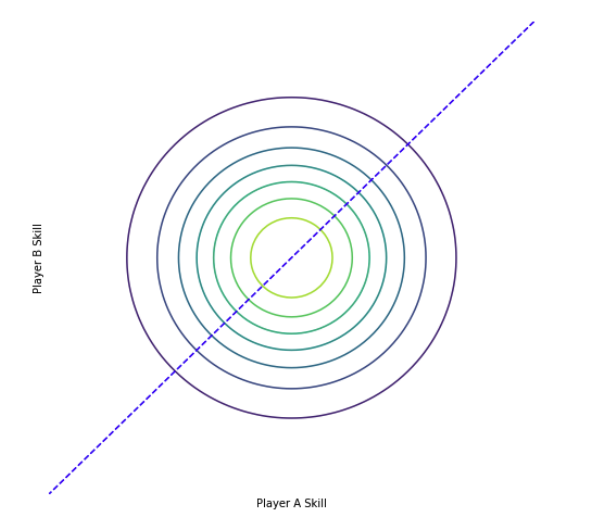
\includegraphics[width = .4\linewidth]{figures/section8/figure_8_1.png}
        \caption{Contour plot between two players}
        \label{fig:prior_trueskill}
    \end{figure}
    The above graph shows the contour graph between the two players. Since we assume both players follows Gaussian distribution, we are uncertain about players skills and hence we observe perfect "circles." Each contour represent different values of pdf. It goes higher when we move to the center. The blue dashed line represent equal skills between the two players. \href{https://en.wikipedia.org/wiki/Multivariate_normal_distribution#/media/File:Multivariate_Gaussian.png}{Here} is 3D view of the bivariate Gaussian distribution.
    \begin{figure}[H]
        \centering
        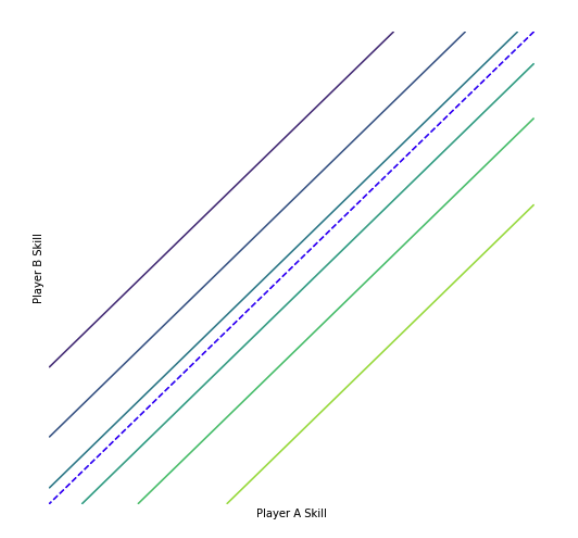
\includegraphics[width = .4\linewidth]{figures/section8/figure_8_2.png}
        \caption{2D projection of likelihood}
        \label{fig:likelihood_trueskill}
    \end{figure}
    The above graph shows the 2D projection of the likelihood $p(i\:\text{i beats j}|z_i,z_j)=\sigma(z_i-z_j)$.
    \begin{figure}[H]
        \centering
        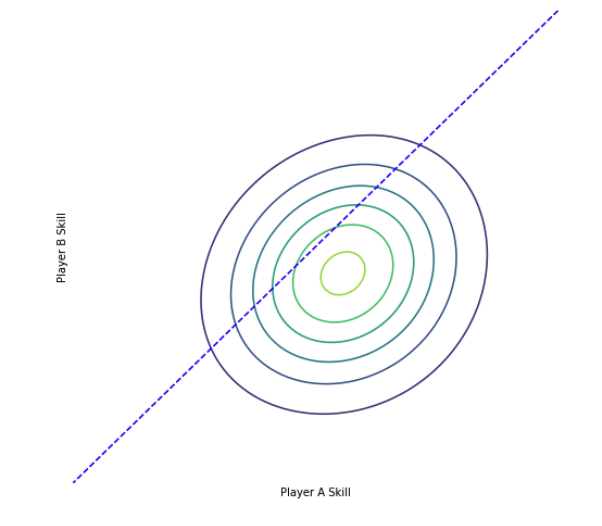
\includegraphics[width = .4\linewidth]{figures/section8/figure_8_3.png}
        \caption{The posterior}
        \label{fig:posterior_trueskill}
    \end{figure}
    The contours are not perfect "circles" anymore, which are not Gaussian anymore. However, the center moves to the left and we conclude that the guess player A is better than B.
\end{example}
\subsection{Kullback-Leibler divergence}
From the TrueSkill model, the normalizing factor $p(x)=\int p(x,z)dz$ is intractable when $z$ is high-dimensional. To estimate $p(x)$, like previously explained, our procedure is to approximate it using a simpler distribution $q(x)$. We measure the closeness/similarity between $p$ and $q$ using \textbf{KL Divergence}.
$$\mathrm{KL}(q(z) \| p(z | x))=\int q(z) \log \frac{q(z)}{p(z | x)} d z=\underset{z \sim q}{\mathbb{E}} \log \frac{q(z)}{p(z | x)}$$
\begin{itemize}
    \item $\mathrm{KL}(q \| p) \geq 0$
    \item $\mathrm{KL}(q \| p)=0 \Leftrightarrow q=p$
    \item $\mathrm{KL}(q \| p) \neq \mathrm{KL}(p \| q)$
    \item KL divergence is not a metric, since it is not symmetric.
\end{itemize}
$\mathrm{KL}(q \| p)$ and $\mathrm{KL}(p \| q)$ corresponds to different projection.

\subsubsection*{Information (I-) Projection}
For I-projection, we want to find the $\star{q}$ such that:
$$q^*=\arg \min _{q \in Q} \mathrm{KL}(q \| p)=\mathbb{E}_{x \sim q(x)} \log \frac{q(x)}{p(x)}$$
\begin{itemize}
    \item We want to minimize KL divergence from $q$ (approximating distribution) to $p$ (target distribution).
    \item We focuses on the simpler model that captures the main features of the target distribution.
    \item Thus I-projection will not yield the correct moments.
\end{itemize}
\begin{figure}[H]
    \centering
    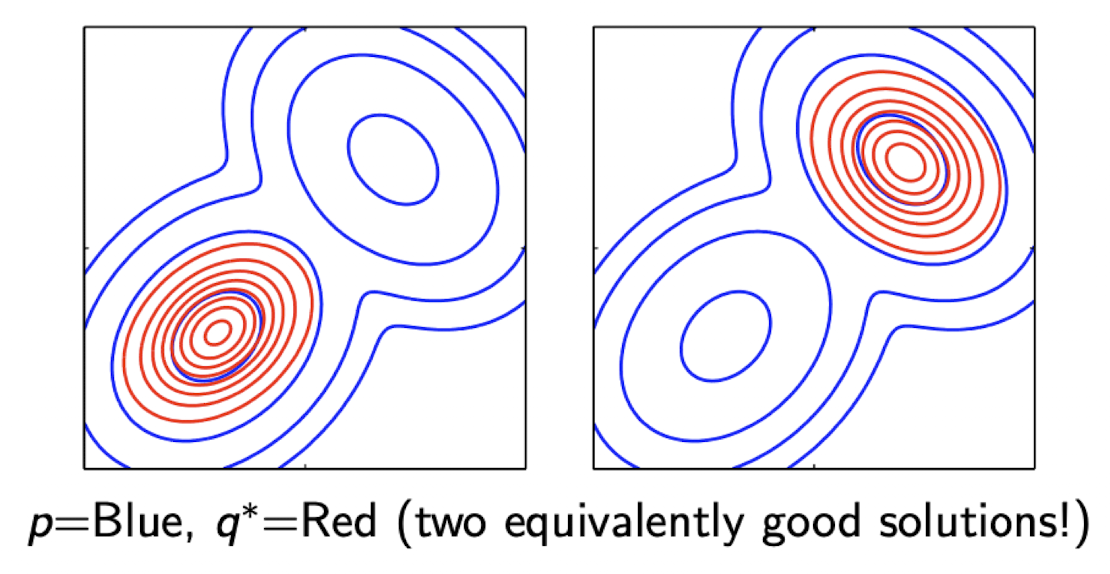
\includegraphics[width = .4\linewidth]{figures/section8/figure_8_4.png}
    \caption{An example of I-projection}
    \label{fig:I-projection}
\end{figure}


\subsubsection*{Moment (M-) Projection}
For I-projection, we want to find the $\star{q}$ such that:
$$q^*=\arg \min _{q \in Q} \mathrm{KL}(p \| q)=\mathbb{E}_{x \sim q(x)} \log \frac{p(x)}{q(x)}$$
\begin{itemize}
    \item We want to minimize KL divergence from $p$ (target distribution) to $p$ (approximating distribution).
    \item We Preserves the characteristics of $p$ as much as possible in $q$
    \item Thus M-projection will yield the correct moments.
\end{itemize}
\begin{figure}[H]
    \centering
    \caption{An example of M-projection}
    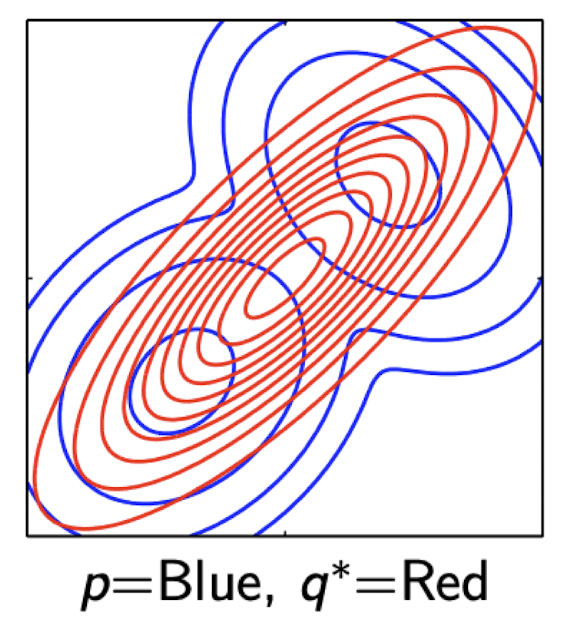
\includegraphics[width = .3\linewidth]{figures/section8/figure_8_5.png}
    \label{fig:M-projection}
\end{figure}

\subsection{Mean-field approach}
We know that MRF can be written as exponential families:
$$
p(x | \theta)=\exp \left\{\sum_{C \in \mathcal{C}} \phi_C\left(x_C\right)-\log Z(\theta)\right\}
$$
By performing I-projection:
$$\mathrm{KL}(q \| p)=\mathbb{E}_{x \sim q(x)} \log \frac{q(x)}{p(x | \theta)}=\mathbb{E}_{x \sim q(x)}\left[\log q(x)-\sum_{C \in \mathcal{C}} \phi_C\left(x_C\right)+\log Z(\theta)\right]$$
Denote \textbf{entropy} as $H(p)=-\mathbb{E}_{x \sim p(x)} \log p(x)$, which measures the uncertainty in $p$
$$\arg \min _{q \in Q} \mathrm{KL}(q \| p)=\arg \max _{q \in Q}\left\{\sum_{C \in \mathcal{C}} \mathbb{E}_q\left[\phi_C\left(x_C\right)\right]+H(q)\right\}$$
Using the KL divergence, we need to define a nice set of $Q$, if $p\in Q$, then we are done. However, it is nearly impossible and we should take \textbf{mean-field approach}.\\

The key assumption for mean-field approach is that we assume $Q$ is composed of those distributions that factor out:
$$q(x)=\prod_{i \in V} q_i\left(x_i\right)$$
Therefore, $q^*$ is now equivalent to:
$$
q^*=\arg \max _{q \in Q} \sum_{C \in \mathcal{C}} \underbrace{\sum_{x_C} q_C\left(x_C\right) \phi_C\left(x_C\right)}_{\mathbb{E}_q\left[\phi_C\left(x_C\right)\right]}+H(q)
$$
For the entropy:
$$
\begin{aligned}
H(q) & =\mathbb{E}_q[-\log q(x)]=-\sum_x q(x) \log q(x)=-\sum_x q(x)\left[\sum_i \log q_i\left(x_i\right)\right] \\
& =-\sum_i \sum_x\left[q_i\left(x_i\right) \log q_i\left(x_i\right)\right] \frac{q(x)}{q_i\left(x_i\right)}=-\sum_i \sum_{x_i}\left[q_i\left(x_i\right) \log q_i\left(x_i\right)\right] \sum_{x_i} \frac{q(x)}{q_i\left(x_i\right)} \\
& =-\sum_i \sum_{x_i}\left[q_i\left(x_i\right) \log q_i\left(x_i\right)\right]=\sum_i H\left(q_i\right)
\end{aligned}
$$
This tells us the general result on how to find $H(q)$ from each $q_i$, we can thus write everything as a function of $q_i$ for $i \in V$.

\subsection{Evidence Lower Bound (ELBO)}
\begin{align*} 
    \mathrm{KL}\left(q_\phi(z) \| p(z \mid x)\right) & =\underset{z \sim q_\phi}{\mathbb{E}} \log \frac{q_\phi(z)}{p(z \mid x)} \\ 
    & =\underset{z \sim q_\phi}{\mathbb{E}}\left[\log \left(q_\phi(z) \cdot \frac{p(x)}{p(z, x)}\right)\right] \\ 
    & =\underset{z \sim q_\phi}{\mathbb{E}}\left[\log \frac{q_\phi(z)}{p(z, x)}\right]+\underset{z \sim q_\phi}{\mathbb{E}} \log p(x) \\ 
    & :=-\underbrace{\mathcal{L}(\phi)}_{ELBO}+\log p(x)
\end{align*}
Further simplification, we have:
\begin{align*}
\mathcal{L}(\phi)&=\underset{z \sim q_\phi}{\mathbb{E}}\left[\log p(z, x)-\log q_\phi(z)\right]\\
&=\underbrace{\underset{z \sim q_\phi}{\mathbb{E}}[\log p(z, x)]}_{\text{expected log-join}}+\underbrace{\underset{z \sim q_\phi}{\mathbb{E}}\left[-\log q_\phi(z)\right]}_{\text{entropy}}
\end{align*}
Rearrange, we have:
$$\mathcal{L}(\phi)+\underbrace{\mathrm{KL}\left(q_\phi(z) \| p(z \mid x)\right)}_{\geq 0}=\log p(x)$$
$$\Rightarrow \mathcal{L}(\phi)\leq \log p(x)$$
Therefore, maximizing the ELBO is equivalent to minimize the KL divergence.